\section{Introducción}

\subsection{Big Data en Astronomía}

En los últimos años, los ámbitos empresarial, científicos y de administración
han estado haciendo frente a la avalancha de datos proveniente de distintas
fuentes asociadas a cada investigación, concepto que se ha definido como
\emph{Big Data}.
Por su simple denominación, se entiende que trata de la manipulación de grandes
volúmenes de información, los cuales no son sencillos de procesar con las herramientas
y procedimientos tradicionales.
Con la idea de procesamiento de información a gran escala,
la evolución de los métodos y recursos habitualmente utilizados
ha sido la responsable de ser capaces de manipular grandes volúmenes de datos,
los cuales pueden llegar a ser del orden de TeraBytes a ZetaBytes.
Adicionalmente, no sólo estamos tratando con grandes volúmenes de datos
de manera estacionaria, si no que la frecuencia con la cual éstos son generados,
crea nuevos componentes críticos para las el desarrollo de soluciones,
como lo son el almacenamiento, variabilidad de formato, y tiempo de respuesta.
Es en el área de la astronomía, donde podemos ver el concepto de \emph{Big Data}
en una situación real, en las cuales las instalaciones de última generación
recientes, como el Atacama Large Millimeter/submillimeter (ALMA),
y las que están en construcción, como el Large Synoptic Survey Telescope (LSST) y el
Square Kilometer Array (SKA)
producen y producirán datos de gran escala, proyectándose que para el año 2020
serán más de 60 PetaBytes de información accesible para la comunidad astronómica.

Considerando todos los aspectos técnicos y tecnológicos de la manipulación
de grandes volúmenes de datos en los ejemplos anteriormente señalados, requieren
el desarrollo de sistemas específicos para cada uno de ellos,
los cuales consideran aspectos de captura, almacenamiento, distribución, gestión
y análisis de la información.

\emph{Big Data} no es una tecnología en sí misma, sino más bien un planteamiento de
trabajo para la obtención de valor y beneficios de los grandes volúmenes de
datos que se están generando hoy en día. Se deben contemplar aspectos como:

\begin{itemize}
    \item Cómo capturar, gestionar y explotar
    \item Cómo asegurar, verificar validez y fiabilidad.
    \item Cómo compartir para obtener mejoras y beneficios.
    \item Cómo comunicar para facilitar la toma de decisión y posteriores análisis.
\end{itemize}

\subsection{Observatorios en Chile}

Las privilegiadas condiciones atmosféricas hacen de Chile uno de los lugares
más propicios para la realización de investigaciones científicas en astronomía.

Existen más de una docena de instalaciones astronómicas de gran envergadura a
lo largo de nuestro territorio nacional {\bf ref observatorios chile}, como por
ejemplo, el anteriormente nombrado ``Atacama Large Milimeter/submilimeter
Array'' (ALMA), el ``Very Large Telescope'' (VLT), y en los próximos años el
``European Extremely Large Telescope'' (E-ELT), con el cual se estima que el
$60\%$ de la observación astronómica mundial se realice en Chile.

Una de las condiciones que se establecen a nivel país, es que el $10\%$ del
tiempo de observación pertenece a la comunidad astronómica chilena, lo cual
justifica la necesidad a nivel país del desarrollo de una plataforma
astroinformática para una inteligente administración y análisis.

La necesidad de un sistema con éstas características no es algo nuevo, debido
que desde el $2002$ se planteó éste tipo de problemática, lo cual sugirió la
creación de un Observatorio Virtual (VO, por sus siglas en inglés) como una
solución.

El VO es una iniciativa internacional que permite el acceso de datos
astronómicos, a cargo de centros especializados para su almacenamiento y
procesamiento, a los cuales pueden acceder tanto astrónomos, como personas
comunes.  Con la estandarización de métodos e información es posible estudiar
los registros astronómicos sin requerimientos físicos de instrumentos y
localización.

\subsection{¿Por qué es nuevo?}
VO con datos de ALMA.

Resumen de lo importante del paper.

%\subsection{IVOA Standards}


\subsection{ALMA + Cubos + Formatos propios}

ALMA Consiste en recolectar una señal proveniente del cielo usando dos o más
antenas y combinarlas para analizar la señal y así obtener información de la
fuente de la emisión (ya sea una estrella, planeta, o galaxia), para ello usa
66 atenas ubicadas en Chajnantor a más de 5 mil metros de altura. Al combinar
ondas de radio capturadas por dos o más antenas, es posible obtener datos de
alta precisión y actualmente estas ondas de radio van entre frecuencias de 84
GHz y 950 GHz (ALMA Band 3 - ALMA Band 10). 

Del punto de vista de producción de datos, este proceso genera cubos en tres
dimensiones dadas por: 2 ejes de posición y un eje de frecuencia
\ref{fig:cube}. La particularidad de estos cubos de datos es su tamaño dada por
la alta precisión del observatorio, por lo que son datos de gran esacala (orden
de GB y TB).

\begin{figure}[ht]
    \centering
    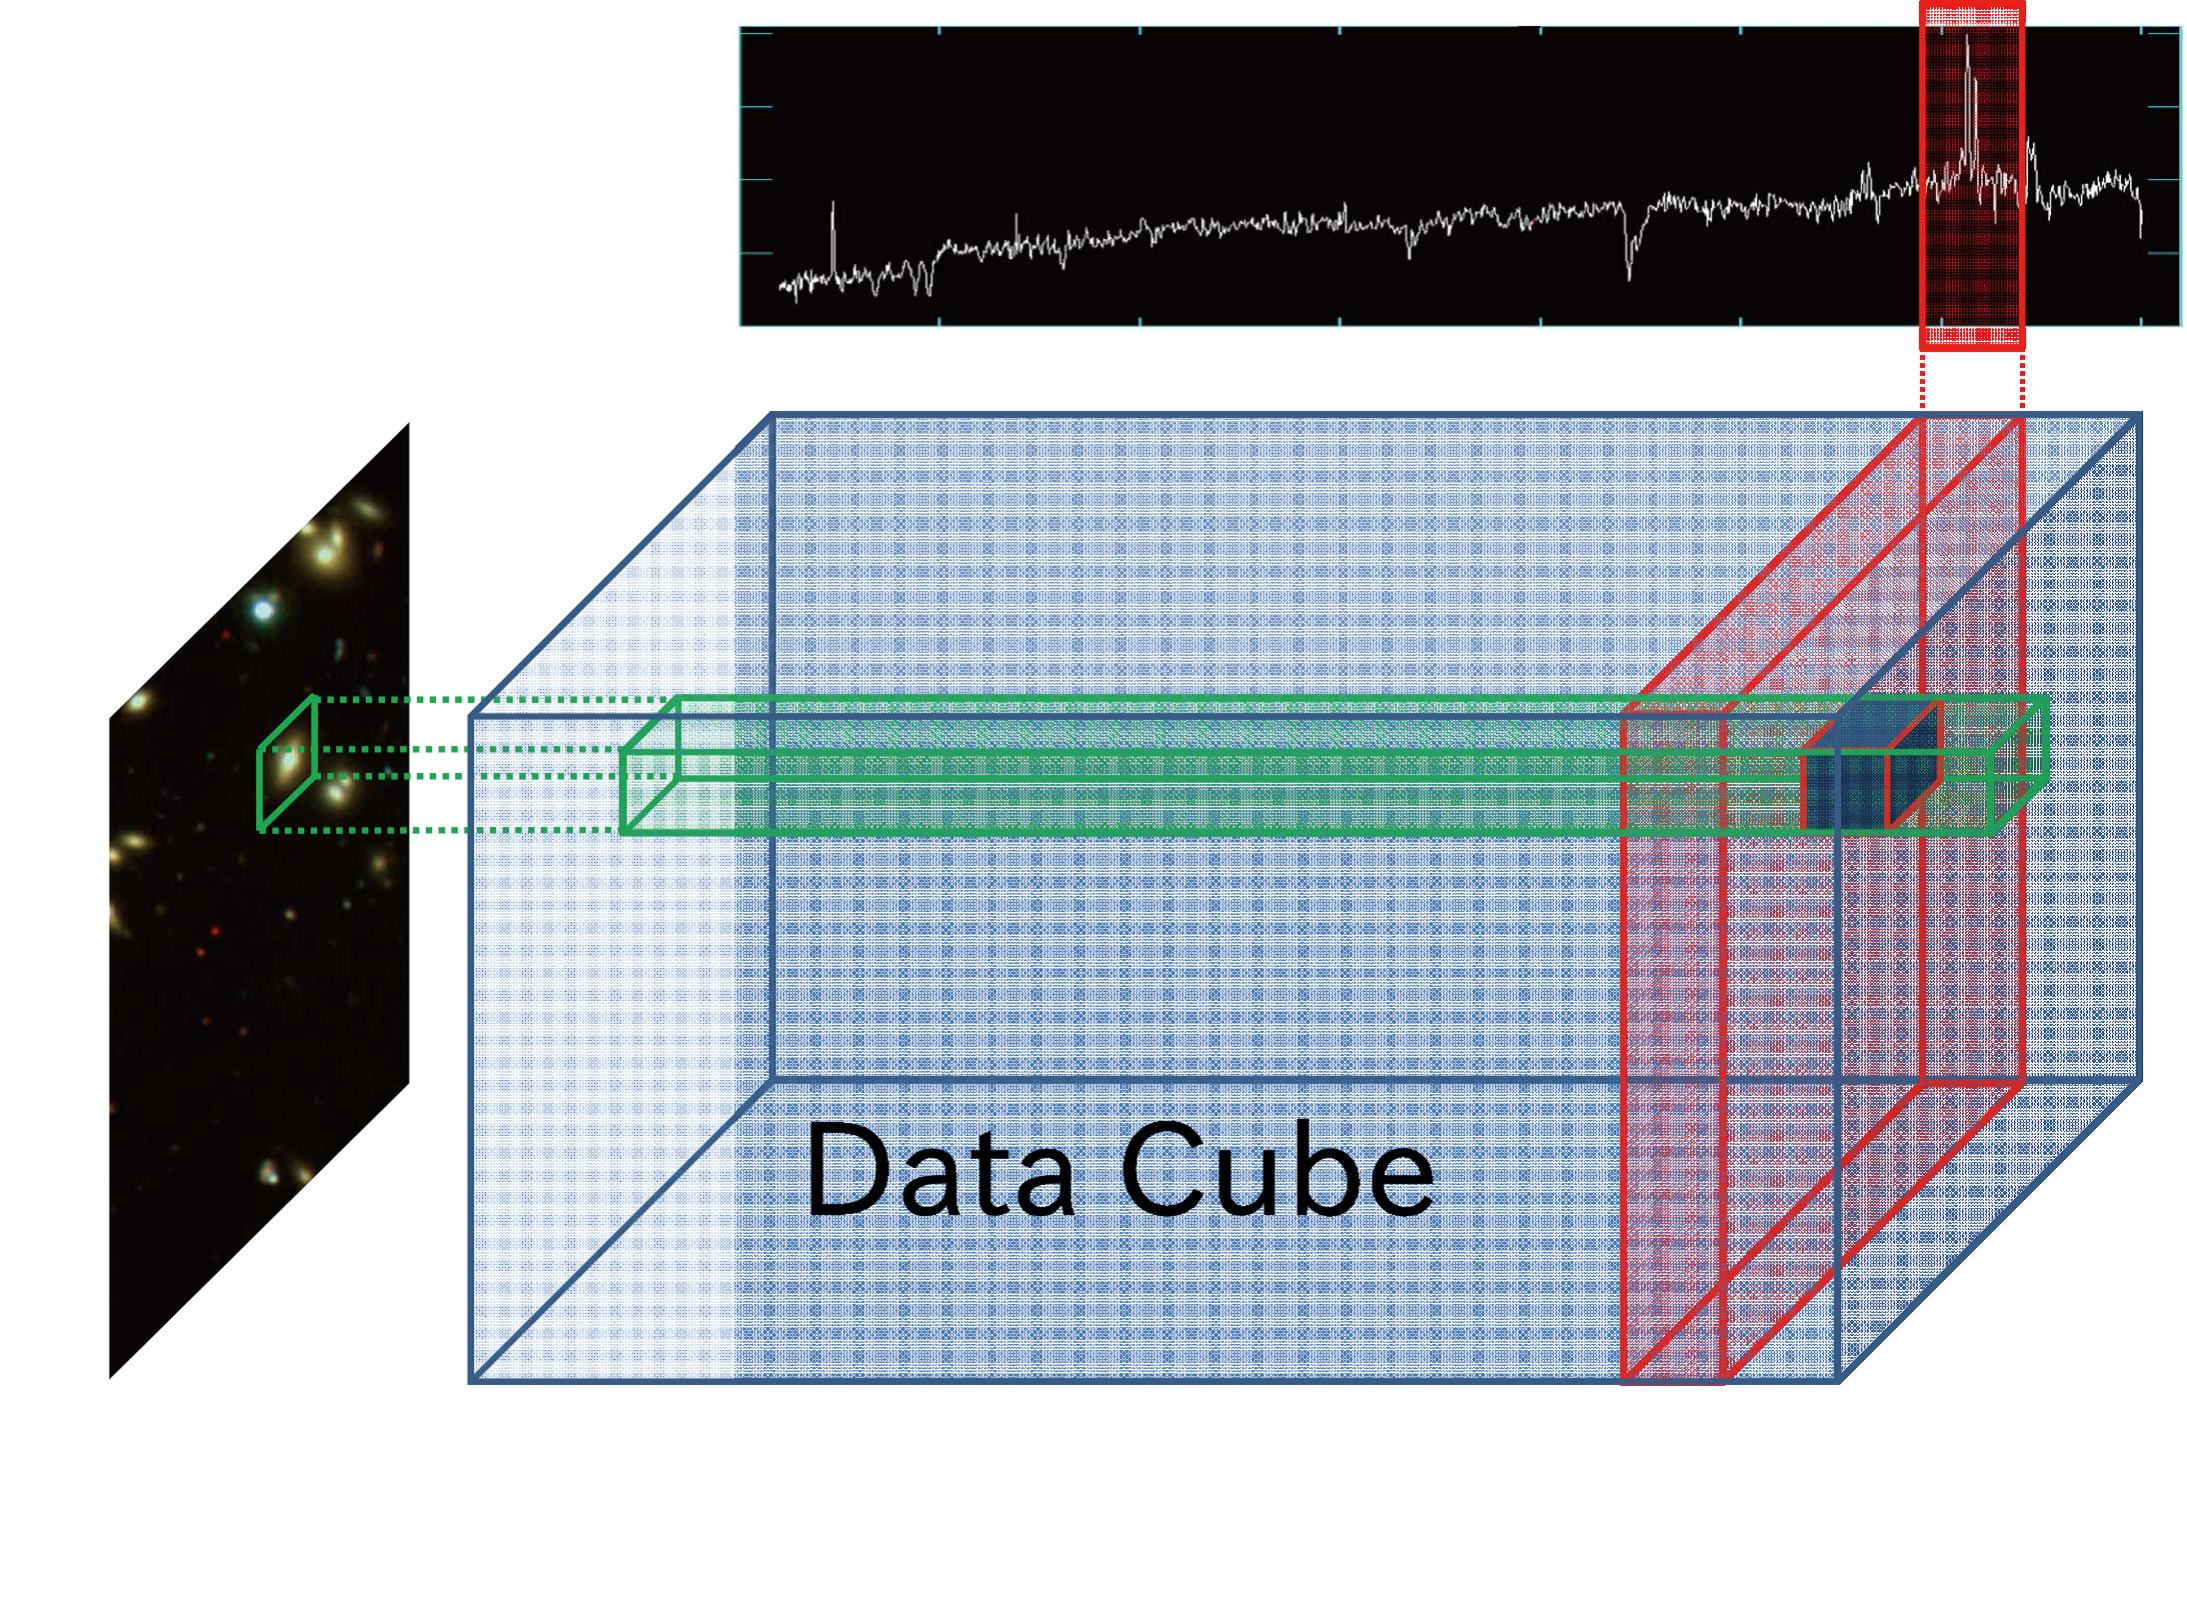
\includegraphics[width=0.45\textwidth]{images/cube.png}
    \caption{Estructura de cubos de datos de ALMA \cite{dent20132}}
    \label{fig:cube}
\end{figure}

En cuanto a formatos de datos en astronomía, todos se rigen por una estructura
similar compuesta por metadatos (información que describe los datos) mas datos
binarios. ALMA posee dos modelos de datos especiales:
\begin{description}
    \item[ALMA Science Data Model:] \hfill \\
        Formato en XML diseñado para guardar los metadatos obtenidos del
        proceso de observación y generar un link hace los datos binarios.
    \item[Measurement Set:] \hfill \\
        Formato basado en tablas binarias (1 principal y varias secundarias),
        el que también guarda metadata y datos binarios. Este formato se usa
        para reducir en Common Astronomy Software Applications (CASA), software
        creado por ALMA.
\end{description}
